\chapter{Kiểm thử và đánh giá}
\label{chap:kiem-thu}

Chương này nói về cách kiểm chứng nền tảng và những gì đo được. Con số nào cũng lấy từ một lần chạy có lưu vết trong kho mã, còn câu lệnh để chạy lại nằm ở Phụ lục~\ref{app:tai-tao}.

\section{Chiến lược kiểm thử}

Kiểm thử được sắp theo hình kim tự tháp~\cite{cohn2009}, gồm bốn tầng:

\begin{enumerate}
\item \textbf{Kiểm thử đơn vị} cho tầng miền, nơi hàm thuần không cần giả lập gì, và cho dịch vụ ứng dụng, nơi Repository, LLM và sandbox được thay bằng bản trong bộ nhớ.
\item \textbf{Kiểm thử tích hợp HTTP.} Dựng một ứng dụng Nest thật với guard, interceptor, controller thật, dữ liệu để trong bộ nhớ, rồi gọi vào qua HTTP.
\item \textbf{Kiểm thử đầu cuối} trên hạ tầng thật, gồm API đã build, PostgreSQL, Redis, nginx, một LLM kịch bản tương thích OpenAI và trình duyệt Playwright cho giao diện. Mỗi lần chạy có một tệp điều khiển, in ra một dòng cho mỗi kiểm tra và trả mã lỗi khác 0 nếu có kiểm tra hỏng.
\item \textbf{Kiểm thử tải} với ngân sách thời gian phản hồi cho từng endpoint.
\end{enumerate}

LLM kịch bản được dùng có chủ đích. Máy chủ này trả lời tuỳ theo nội dung lời nhắc, chẳng hạn dự án có tên bắt đầu bằng ``Legacy'' sẽ nhận bản mã đầu tiên vi phạm phân lớp. Độ trễ của nó tăng theo độ dài lời nhắc, và tên mô hình nó dùng có trong bảng giá. Nhờ vậy thời lượng và chi phí khác nhau giữa các dự án, đủ để huấn luyện mô hình dự báo, mà chạy lại bao nhiêu lần cũng ra đúng một kết quả.

\section{Kiểm thử tự động và độ bao phủ}

Bảng~\ref{tab:ket-qua-test} là kết quả của các bộ kiểm thử tự động. Mười lăm kiểm thử bị bỏ qua đều thuộc phần sandbox container, vì máy đo không có Docker daemon.

\begin{table}{Kết quả kiểm thử tự động}
\label{tab:ket-qua-test}
\begin{tabularx}{\textwidth}{|P{3.4cm}|L|}
\hline
\textbf{Bộ kiểm thử} & \textbf{Kết quả} \\ \hline
API (Jest) & 50 bộ, \textbf{707 đạt}, 15 bỏ qua, 0 thất bại \\ \hline
Web (Vitest) & 11 tệp, 44 đạt, chạy lại sau khi nâng cấp Ant Design 6 \\ \hline
Biên dịch & \code{nest build} 0 lỗi, \code{tsc --noEmit} của web 0 lỗi, \code{vite build} thành công \\ \hline
\end{tabularx}
\end{table}

Ngưỡng độ bao phủ được khai trong cấu hình Jest, nên chưa đạt thì lệnh \code{npm run test:cov} tự báo lỗi. Bảng~\ref{tab:bao-phu} đặt số đo cạnh ngưỡng.

\begin{table}{Độ bao phủ mã và ngưỡng}
\label{tab:bao-phu}
\small
\begin{tabular}{|l|r|r|r|r|c|}
\hline
\textbf{Phạm vi} & \textbf{Dòng} & \textbf{Lệnh} & \textbf{Hàm} & \textbf{Nhánh} & \textbf{Ngưỡng (dòng/lệnh/hàm/nhánh)} \\ \hline
Tầng miền & \textbf{97,1\%} & \textbf{96,2\%} & \textbf{97,0\%} & \textbf{88,1\%} & 90 / 90 / 90 / 85 \\ \hline
Toàn API & 77,8\% & 77,7\% & 74,4\% & 63,5\% & sàn 70 / 70 / 64 / 55 \\ \hline
\end{tabular}
\end{table}

Ngưỡng 90\% chỉ áp cho tầng miền chứ không áp cho cả API. Tầng miền chứa quy tắc nghiệp vụ, còn controller và phần nối với NestJS phần lớn là mã khung, đòi 90\% ở đó thì thực ra là đi kiểm thử lại framework. Tuy vậy, toàn API vẫn có một ngưỡng sàn để độ bao phủ không tụt dần theo thời gian.

\section{Kiểm thử đầu cuối}

Bảng~\ref{tab:e2e} tóm tắt ba lần chạy đầu cuối chính. Lần nào cũng bắt đầu từ cơ sở dữ liệu trống. Ngoài ba lần này còn có các lần chạy riêng cho bộ máy quy trình (quy trình con, ghim phiên bản, ảnh chụp và khôi phục, nhánh song song) và cho hệ thống tác tử (lưu sản phẩm OOAD, QC chạy kiểm thử, cơ chế học, lập trình cặp).

\begin{table}{Ba lần chạy kiểm thử đầu cuối chính}
\label{tab:e2e}
\small
\begin{tabularx}{\textwidth}{|P{3.4cm}|L|r|}
\hline
\textbf{Lần chạy} & \textbf{Nội dung} & \textbf{Kết quả} \\ \hline
Triển khai và trình diễn & Cấu hình production qua nginx, dữ liệu trình diễn, phân quyền, phê duyệt, xuất PDF, phân tích, kiểm toán, nhà cung cấp LLM & \textbf{24/24} \\ \hline
Phân tích, dự báo, chất lượng mã & 8 dự án chạy hết quy trình OOAD, rồi 3 lượt chạy khi mô hình của Marketing ngừng hoạt động, dùng bộ nhận webhook thật & \textbf{21/21} \\ \hline
Bảo mật, kiểm toán, tích hợp & Vai trò và quyền, nhật ký kiểm toán, khoá API, giới hạn tần suất, webhook ký HMAC, xuất dữ liệu, báo cáo & \textbf{44/44} \\ \hline
\end{tabularx}
\end{table}

Lần chạy triển khai kiểm tra những thứ mà kiểm thử đơn vị không nhìn thấy được:

\begin{itemize}
\item \code{prisma migrate deploy} dựng đúng lược đồ trên cơ sở dữ liệu trống qua ba migration, trong đó có migration cho bảng nhà cung cấp LLM. Lược đồ thu được không lệch so với mô hình (\code{prisma migrate diff --exit-code} trả 0).
\item API ở chế độ production từ chối khởi động khi cấu hình sai (thiếu \code{JWT_SECRET} và \code{CORS_ORIGIN}, khoá LLM là \code{CHANGE_ME}). Tiến trình thoát với mã 1 và in ra đủ cả ba lỗi.
\item Qua nginx, điểm kiểm tra tình trạng báo cơ sở dữ liệu, Redis và cổng LLM đều \textit{healthy}. Dừng PostgreSQL thì \code{/api/health} trả 503 trong khi \code{/api/health/live} vẫn trả 200; bật lại PostgreSQL thì kết quả trở về 200.
\item Swagger tắt khi \code{ENABLE_SWAGGER=false}, còn CORS chỉ trả header cho nguồn gốc đã cấu hình.
\item Kết nối WebSocket qua nginx nhận token hợp lệ và ngắt kết nối khi gặp token giả.
\item Người xem không tạo được dự án, không phê duyệt được qua REST và cũng không phê duyệt được qua WebSocket. Lỗ hổng ở kênh WebSocket được tìm ra và vá ngay trong lần chạy này (mục~\ref{sec:loi}).
\item Một phê duyệt chỉ trả lời được một lần, lần thứ hai nhận 409. Tài khoản tự đăng ký nhận vai trò người xem. Cổng LLM trong cấu hình được nhập thành nhà cung cấp đầu tiên với 19 mô hình, và API không trả khoá của nhà cung cấp này.
\item Sau khi thành viên hội đồng quản trị phê duyệt, CEO đóng dự án, và nhật ký kiểm toán có đủ \code{auth.login}, \code{project.create}, \code{approval.requested}, \code{approval.approve}, \code{access.denied}, \code{quality.gate.evaluated}, \code{workflow.completed}.
\end{itemize}

\begin{figure}{Hộp thoại phê duyệt của dự án Clinic Booking}
\label{fig:phe-duyet}
\centering
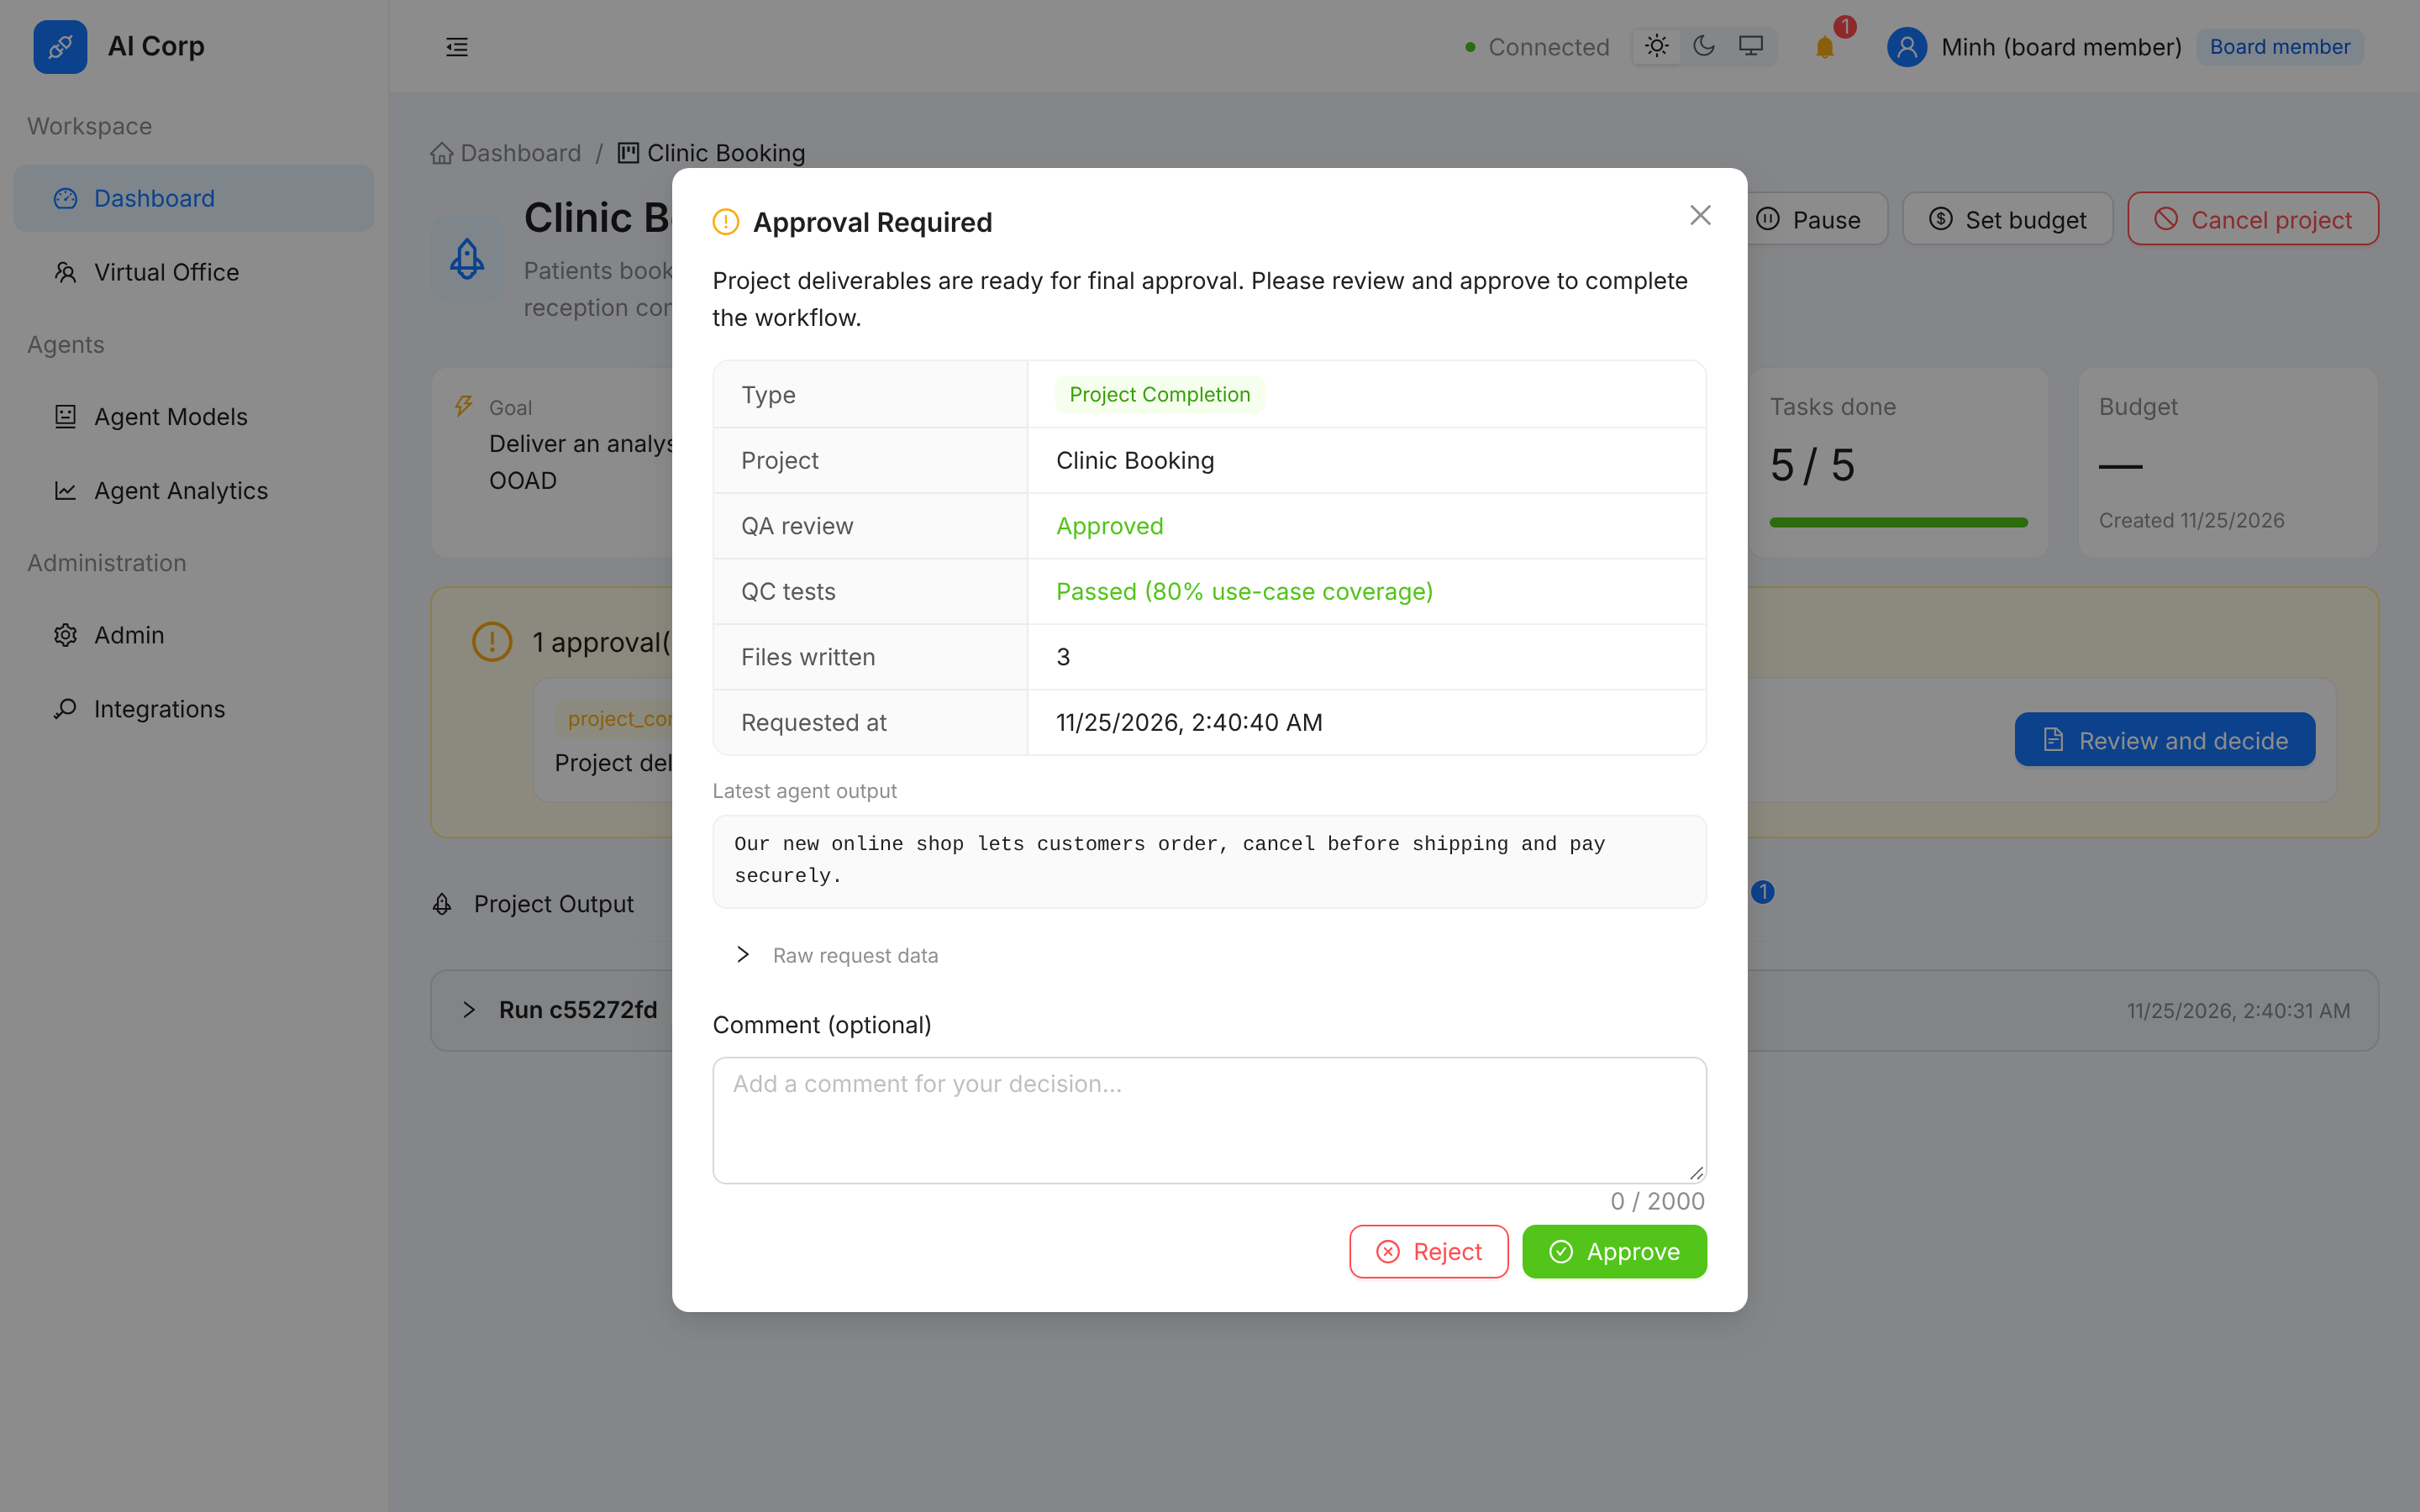
\includegraphics[width=\textwidth]{anh/approval.png}
\end{figure}

Hình~\ref{fig:phe-duyet} là hộp thoại mà thành viên hội đồng quản trị thấy khi bấm \textit{Review and decide} trên dự án Clinic Booking. Phần tóm tắt cho biết QA đã duyệt, QC đã chạy kiểm thử đạt với 80\% use case được bao phủ, kèm đầu ra mới nhất của tác tử. Dữ liệu thô của yêu cầu vẫn xem được nhưng được thu gọn lại.

\section{Thời gian xử lý một nút quy trình}

Theo yêu cầu phi chức năng, mỗi nút quy trình phải xong trong 2 giây, không tính độ trễ LLM, vì độ trễ đó tuỳ nhà cung cấp và nền tảng không điều khiển được. Bảng~\ref{tab:thoi-gian-nut} là thời lượng của 43 bước tác tử trong lần chạy triển khai. LLM kịch bản trả lời sau 20~ms cộng 1~ms cho mỗi 25 ký tự lời nhắc, nên các con số vẫn chứa một phần độ trễ giả lập.

\begin{table}{Thời lượng bước tác tử theo vai trò}
\label{tab:thoi-gian-nut}
\begin{tabular}{|l|r|r|r|r|}
\hline
\textbf{Vai trò} & \textbf{Số bước} & \textbf{p50 (ms)} & \textbf{p95 (ms)} & \textbf{Lớn nhất (ms)} \\ \hline
CEO & 10 & 75 & 100 & 100 \\ \hline
BA & 5 & 107 & 121 & 121 \\ \hline
Architect & 5 & 582 & 607 & 607 \\ \hline
PM & 4 & 105 & 110 & 110 \\ \hline
DEV & 5 & 614 & 632 & 632 \\ \hline
QC & 5 & 1\,642 & 1\,726 & 1\,726 \\ \hline
QA & 5 & 259 & 279 & 279 \\ \hline
Marketing & 4 & 75 & 81 & 81 \\ \hline
\textbf{Tất cả} & \textbf{43} & \textbf{110} & \textbf{1\,642} & p99: \textbf{1\,726} \\ \hline
\end{tabular}
\end{table}

Nút nào cũng xong dưới 2 giây. Kết quả gần như trùng với lần đo trước khi bộ máy thêm bước kiểm tra ngân sách trước mỗi nút (p50 108~ms, p95 1\,687~ms), tức là bước kiểm tra này hầu như không làm hệ thống chậm đi. QC chậm nhất vì tác tử này chạy thật bộ kiểm thử Jest của dự án sinh ra. Architect và DEV chậm hơn các vai trò còn lại vì phải ghi nhiều tệp và chạy phân tích tĩnh.

\section{Hiệu năng dưới tải}

Kiểm thử tải dùng một script không cần thư viện ngoài, đóng vai người dùng bảng điều khiển: xem danh sách và chi tiết dự án, công việc, báo cáo chi phí, phân tích tác tử, dự báo và chất lượng mã. Mỗi endpoint có ngân sách thời gian phản hồi p50/p95/p99, mặc định 100/500/1000~ms. Nhóm phân tích, dự báo và chất lượng mã được 300/1500/3000~ms, còn tạo dự án được 500/2000/3000~ms. Tỉ lệ lỗi tối đa là 1\%. Môi trường gồm một tiến trình API ở chế độ production, PostgreSQL và Redis, chạy trên máy 4 lõi dùng chung với bộ sinh tải và LLM kịch bản. Cơ sở dữ liệu bắt đầu với 5 dự án trình diễn và lớn dần khi kịch bản tạo thêm dự án. Kết quả nằm ở Bảng~\ref{tab:tai}.

\begin{table}{Kết quả kiểm thử tải}
\label{tab:tai}
\small
\begin{tabularx}{\textwidth}{|P{4.2cm}|r|r|L|}
\hline
\textbf{Kịch bản} & \textbf{Yêu cầu/s} & \textbf{Lỗi} & \textbf{Kết quả theo ngân sách} \\ \hline
1 người dùng & 184,7 & 0\% & Mọi endpoint trong ngân sách, p50 từ 3 đến 7~ms \\ \hline
20 người dùng, chỉ đọc & \textbf{604,8} & 0\% & Mọi endpoint trong ngân sách, p95 cao nhất 84~ms \\ \hline
20 người dùng, đồng thời tạo 111 dự án & 430,7 & 0\% & Mọi endpoint trong ngân sách, tạo dự án p50 107~ms, p99 177~ms \\ \hline
50 người dùng, tạo 48 dự án & 407,2 & 0\% & Bão hoà: p50 từ 77 đến 312~ms, năm endpoint vượt ngân sách p50 100~ms, mọi p99 dưới 0,7~s \\ \hline
\end{tabularx}
\end{table}

Với 50 người dùng, một tiến trình API đã bão hoà ở khoảng 407 yêu cầu mỗi giây. Theo định luật Little~\cite{little1961}, khi đó mỗi yêu cầu phải nằm trong hệ thống khoảng $50/407 \approx 123$~ms. Đây là giới hạn của một tiến trình đơn chứ không phải do truy vấn chậm. API không giữ trạng thái, vì lượt chạy được điều phối qua BullMQ và PostgreSQL, nên muốn phục vụ nhiều người hơn thì chạy thêm tiến trình.

Lần đo trước đó, trên cơ sở dữ liệu khoảng 120 dự án, cho 201,8 yêu cầu mỗi giây với 20 người dùng và bão hoà ở 178. Hai lần đo có lượng dữ liệu khác nhau nên không so thẳng được, và khoá luận không coi chênh lệch này là cải thiện. Cái so được là kết quả theo ngân sách. Ở cả hai lần, với 20 người dùng, mọi endpoint đều nằm trong hoặc sát ngân sách và không có lỗi. Lần đo trước đã chỉ ra ba lỗi hiệu năng (mục~\ref{sec:loi}). Sửa xong, p50 của endpoint chất lượng mã giảm từ 3,1~s xuống 196~ms trong cùng kịch bản.

\section{Độ chính xác của dự báo}

Sau khi 8 dự án chạy xong, vai trò nào cũng đủ mẫu để dùng mô hình hồi quy. Bảng~\ref{tab:mape} là sai số leave-one-out của dự báo thời gian tác tử.

\begin{table}{Sai số leave-one-out của dự báo thời gian theo vai trò}
\label{tab:mape}
\begin{tabular}{|l|r|}
\hline
\textbf{Vai trò} & \textbf{MAPE (LOO)} \\ \hline
Architect & 3\% \\ \hline
CEO & 5\% \\ \hline
BA & 11\% \\ \hline
DEV & 30\% \\ \hline
\end{tabular}
\end{table}

Xét dự báo lúc bắt đầu của 7 dự án (bỏ dự án đầu vì chưa có lịch sử), sai số tuyệt đối trung bình là 21\% về thời gian và 20\% về chi phí. Phần lớn sai số đến từ một dự án bị QA từ chối và DEV phải làm lại, làm chi phí vượt dự báo 84\%. Các dự án còn lại chỉ lệch từ 0 đến 10\%. Chuyện này dễ hiểu, vì lúc dự án vừa bắt đầu thì không ai biết trước nó có bị từ chối và phải làm lại hay không. Do đó nền tảng lưu cả dự báo lúc bắt đầu lẫn dự báo lúc PM lập kế hoạch, và luôn đặt dự báo cạnh số thực tế (Hình~\ref{fig:du-bao}). Trong hình, dự án Online Bookstore được dự báo 9,4~s và \$0,0587 dựa trên 4 dự án đã xong, còn thực tế đến lúc đó là 9,0~s và \$0,0538.

\begin{figure}{Dự báo công sức, chi phí và điểm chất lượng mã trong tab báo cáo}
\label{fig:du-bao}
\centering
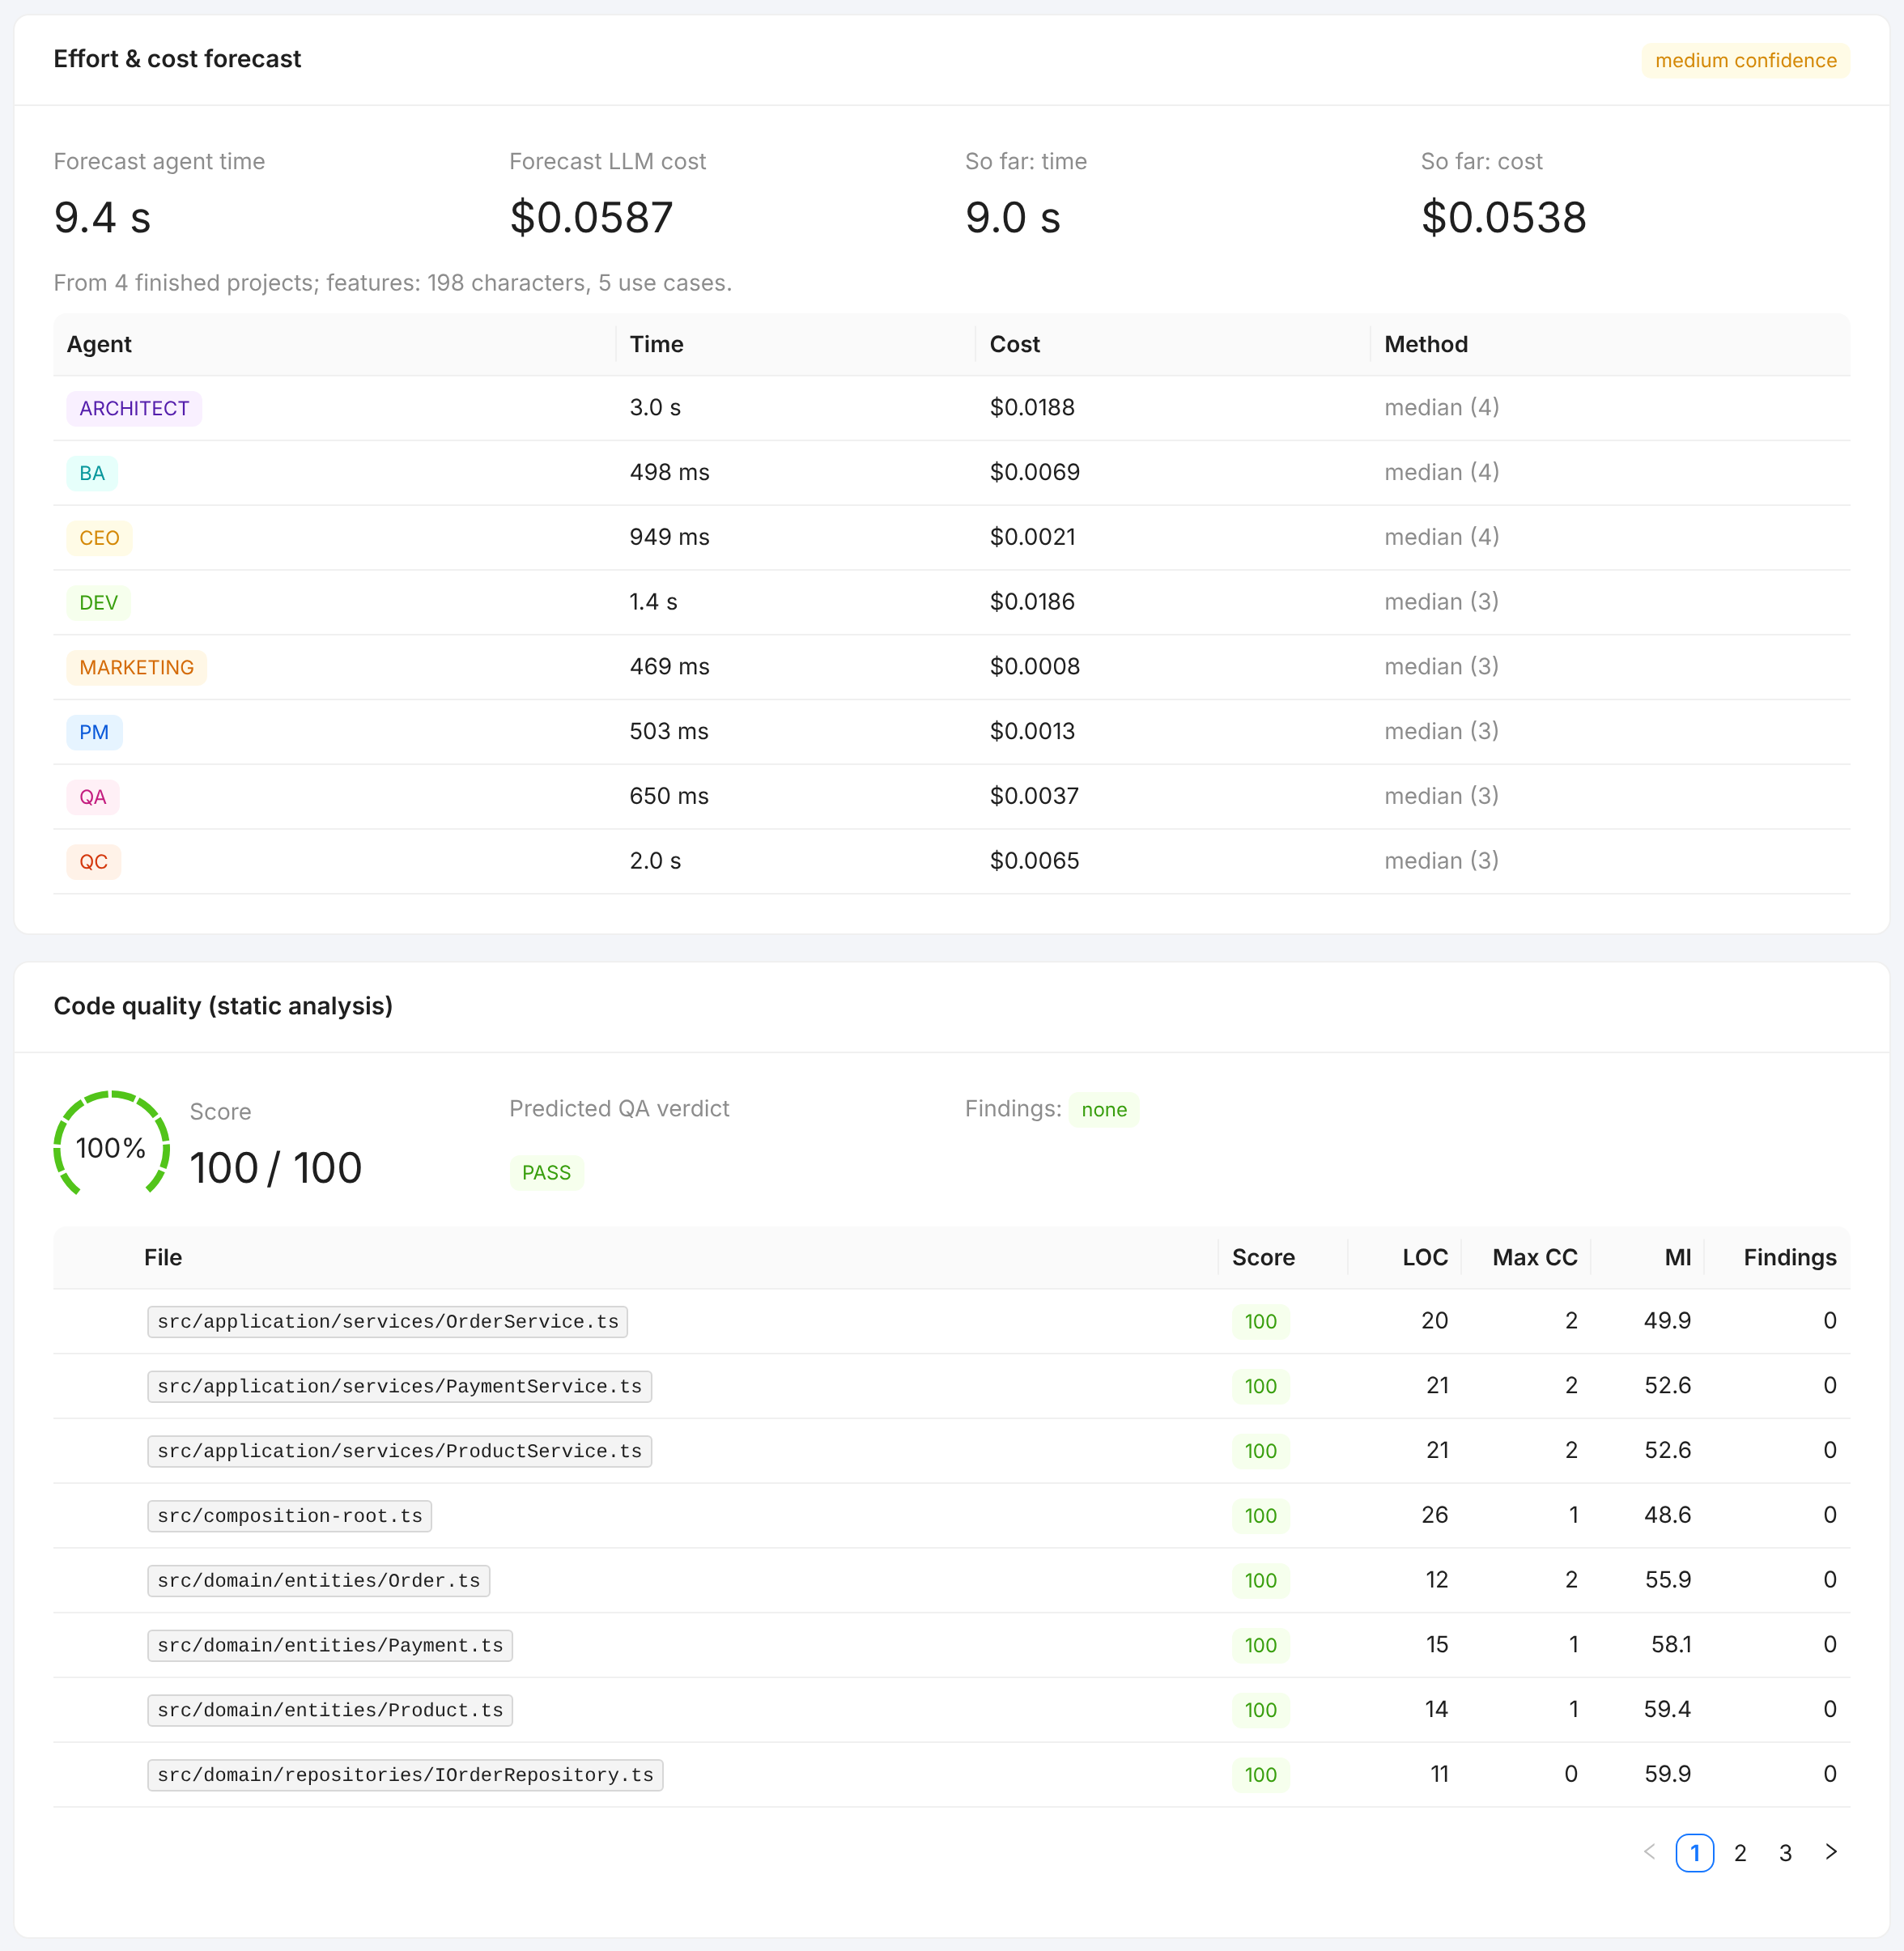
\includegraphics[width=0.85\textwidth]{anh/reports-forecast-quality.png}
\end{figure}

\section{Dự đoán chất lượng mã}

Bảng~\ref{tab:chat-luong-ma} kể lại chuyện gì đã xảy ra ở hai dự án được cài sẵn lỗi, và tổng kết trên tất cả các lần rà soát.

\begin{table}{Dự đoán phán quyết QA từ phân tích tĩnh}
\label{tab:chat-luong-ma}
\small
\begin{tabularx}{\textwidth}{|P{2.6cm}|L|}
\hline
\textbf{Trường hợp} & \textbf{Diễn biến} \\ \hline
Legacy Billing & Mã lần đầu của DEV nhập tầng hạ tầng từ tầng miền, có khoá viết cứng, gọi \code{eval} và dồn quy tắc vào một phương thức dài. Điểm 77 và có vi phạm phân lớp nên dự đoán là \textit{fail}. DEV sửa một vòng, điểm lên 100, bản sửa được giữ và QA duyệt. \\ \hline
Unsafe Portal & Vòng sửa không làm điểm tăng nên bản gốc được giữ. QA thấy \code{eval} trong báo cáo phân tích và trả FAIL. Quy trình quay về DEV, và lần thứ hai thì đạt. \\ \hline
Toàn bộ & Trong 9 lần QA rà soát, 8 lần dự đoán \textit{pass} và được duyệt, 1 lần dự đoán \textit{fail} và bị từ chối. \\ \hline
\end{tabularx}
\end{table}

Độ chính xác 100\% trên 9 lần rà soát phải đọc cẩn thận. Với LLM kịch bản, lỗi được cài sẵn đúng loại mà bộ phân tích bắt được. Con số này cho thấy chuỗi dự đoán, sửa và đối chiếu chạy đúng, nhưng chưa nói được gì về độ chính xác khi dùng LLM thật (mục~\ref{sec:hop-le}).

\section{Nghiên cứu tình huống}

Năm dự án trình diễn được tạo qua API công khai, giống hệt cách một người dùng thật sẽ làm. Mỗi dự án cho thấy một mặt của nền tảng (Bảng~\ref{tab:tinh-huong}). Với LLM kịch bản, cả năm dự án tạo và chạy xong trong khoảng 25 giây.

\begin{table}{Năm dự án trình diễn}
\label{tab:tinh-huong}
\small
\begin{tabularx}{\textwidth}{|P{2.4cm}|P{3.2cm}|L|}
\hline
\textbf{Dự án} & \textbf{Mẫu quy trình} & \textbf{Kết quả} \\ \hline
Online Bookstore & Dự án phần mềm OOAD & 5 use case, 3 thực thể, 3 mẫu thiết kế, đạt cổng OOAD 100\%, 35 tệp, 4 kiểm thử chấp nhận chạy đạt, độ bao phủ use case 80\% (UC-005 bị báo thiếu kiểm thử), có thông báo marketing, hoàn tất \\ \hline
Legacy Billing & Dự án phần mềm OOAD & Phân tích tĩnh phát hiện vi phạm, DEV tự sửa (điểm từ 77 lên 100) trước khi QA rà soát, hoàn tất \\ \hline
Unsafe Portal & Dự án phần mềm OOAD & QA từ chối, quy trình quay về DEV (2 bước DEV, 2 lần QA rà soát), hoàn tất \\ \hline
Library Loans & Chỉ phân tích và thiết kế & Use case, mô hình miền và sơ đồ vượt cổng OOAD, hoàn tất \\ \hline
Clinic Booking & Dự án phần mềm OOAD có phê duyệt & Dừng ở bước phê duyệt. Người xem không duyệt được. Thành viên hội đồng quản trị duyệt xong thì CEO đóng dự án \\ \hline
\end{tabularx}
\end{table}

Ở dự án Online Bookstore, độ bao phủ use case là 80\% chứ không phải 100\%. Chỗ này cho thấy chỉ số không bị làm đẹp. UC-005 không có kiểm thử nào chạy đạt nên không được tính, và ma trận truy vết ghi rõ là nó còn thiếu. Trên Hình~\ref{fig:artifacts}, dòng \textit{UC-005 missing} hiện ngay dưới thanh độ bao phủ.

\section{Lỗi phát hiện nhờ kiểm thử và rà soát}
\label{sec:loi}

Nhờ kiểm thử trên hạ tầng thật, khá nhiều lỗi đã được tìm ra và sửa. Ngoài kiểm thử tự động, lỗi còn lộ ra từ hai nguồn khác. Một là đợt rà soát mã giao diện và logic, trong đó từng màn hình được đọc và so với API mà nó gọi. Hai là lần cài lại từ mã nguồn trên một máy khác. Bảng~\ref{tab:loi} gom lỗi theo nhóm, còn danh sách đầy đủ kèm cách sửa nằm trong kế hoạch dự án và lịch sử thay đổi của kho mã.

\begin{table}{Lỗi phát hiện theo nhóm và theo nguồn}
\label{tab:loi}
\small
\begin{tabularx}{\textwidth}{|P{2.8cm}|L|r|r|r|r|}
\hline
\textbf{Nhóm} & \textbf{Ví dụ tiêu biểu} & \textbf{KT} & \textbf{RS} & \textbf{CĐ} & \textbf{Tổng} \\ \hline
Không khởi động, không chạy được & API không khởi động vì hai chiến lược có tham số hàm tạo mà DI không giải được; migration thiếu 8 bảng; nginx cắt tiền tố \code{/api}; pnpm 8.0 lỗi trên Node 20; bản clone mới không build ra \code{shared-types}; script dữ liệu trình diễn hỏng khi đăng ký mặc định thành người xem & 6 & 0 & 4 & 10 \\ \hline
Bảo mật & Duyệt qua WebSocket bỏ qua kiểm tra quyền và kiểm toán; ba giá trị dự phòng khác nhau cho khoá JWT; tự đăng ký nhận quyền thành viên hội đồng; một phê duyệt trả lời được hai lần; sửa công việc không kiểm tra chủ dự án & 3 & 3 & 0 & 6 \\ \hline
Thiết kế OOAD không được dùng & 4 trên 8 tác tử vẫn chạy luồng cũ nên chiến lược thành mã chết; cổng chất lượng không được đăng ký; sản phẩm tác tử mất sau mỗi lệnh sandbox; quy trình lập kế hoạch trước khi có yêu cầu & 6 & 0 & 0 & 6 \\ \hline
Tính đúng của quy trình và trạng thái & Một máy trạng thái cho mỗi vai trò; nút lỗi để lượt chạy \code{running} mãi; \textit{Pause} chỉ đổi trạng thái dự án; \textit{Resume} ở bước phê duyệt tạo phê duyệt trùng; dự án đã huỷ bị đánh dấu hoàn tất; lý do từ chối không tới được tác tử & 8 & 6 & 0 & 14 \\ \hline
Chi phí và sự kiện & Chi phí LLM của 4 vai trò không được ghi; nút vẫn chạy khi hết ngân sách; cộng chi phí kiểu đọc rồi ghi mất cập nhật khi đồng thời; thiếu sự kiện \code{approval.requested} và \code{workflow.failed} & 4 & 3 & 0 & 7 \\ \hline
Hiệu năng & Phân tích lại mọi tệp ở mỗi yêu cầu (3,1~s); danh sách dự án tải JSON không dùng; bốn truy vấn chạy tuần tự & 3 & 0 & 0 & 3 \\ \hline
Tài liệu và giao diện & 12 trên 39 sơ đồ UML không render được; thẻ dự án luôn hiện 0\%; trang dự án tham gia phòng WebSocket sai payload nên không nhận sự kiện thời gian thực & 3 & 1 & 0 & 4 \\ \hline
\textbf{Tổng} & & \textbf{33} & \textbf{13} & \textbf{4} & \textbf{50} \\ \hline
\end{tabularx}

\vspace{0.2cm}
{\footnotesize KT: kiểm thử, RS: rà soát mã, CĐ: cài đặt mới từ mã nguồn.}
\end{table}

Cả mười ba lỗi do rà soát tìm ra đều nằm trên những luồng mà kiểm thử tự động chưa đi tới. Các kiểm thử đầu cuối chạy quy trình từ đầu tới cuối, nhưng không tạm dừng rồi tiếp tục, không trả lời một phê duyệt hai lần và không cộng chi phí hai lần cùng lúc. Sau khi sửa, mỗi lỗi có một kiểm thử đơn vị riêng (\code{run-control.spec.ts}, \code{approval-and-signup.spec.ts}), và ba hành vi được thêm vào lần chạy đầu cuối triển khai: phê duyệt chỉ trả lời được một lần, tài khoản tự đăng ký chỉ nhận quyền xem, và khoá nhà cung cấp không bị trả về. Chính lần chạy lại ấy cho thấy script tạo dữ liệu trình diễn vẫn mặc định tài khoản tự đăng ký là thành viên hội đồng quản trị.

Lỗ hổng phê duyệt qua WebSocket đáng kể lại, vì trước đó mọi kiểm thử đều đi qua REST. Nó chỉ lộ ra khi kiểm thử đi đúng con đường mà giao diện dùng. Người xem gọi \code{POST /api/approvals/:id/approve} thì nhận 403, nhưng gửi thông điệp \code{human:approval_response} qua WebSocket thì phê duyệt vẫn được chấp nhận, dự án bị đóng và nhật ký kiểm toán không có dòng nào. Bài học thiết kế rút ra là mọi đường ghi dữ liệu phải đi qua cùng một điểm kiểm soát. Sau khi sửa, kênh WebSocket từ chối thông điệp này, giao diện chuyển sang gọi REST, và lần chạy đầu cuối có hẳn một kiểm tra cho trường hợp đó.
